% Options for packages loaded elsewhere
\PassOptionsToPackage{unicode}{hyperref}
\PassOptionsToPackage{hyphens}{url}
\documentclass[
]{article}
\usepackage{xcolor}
\usepackage{amsmath,amssymb}
\setcounter{secnumdepth}{-\maxdimen} % remove section numbering
\usepackage{iftex}
\ifPDFTeX
  \usepackage[T1]{fontenc}
  \usepackage[utf8]{inputenc}
  \usepackage{textcomp} % provide euro and other symbols
\else % if luatex or xetex
  \usepackage{unicode-math} % this also loads fontspec
  \defaultfontfeatures{Scale=MatchLowercase}
  \defaultfontfeatures[\rmfamily]{Ligatures=TeX,Scale=1}
\fi
\usepackage{lmodern}
\ifPDFTeX\else
  % xetex/luatex font selection
\fi
% Use upquote if available, for straight quotes in verbatim environments
\IfFileExists{upquote.sty}{\usepackage{upquote}}{}
\IfFileExists{microtype.sty}{% use microtype if available
  \usepackage[]{microtype}
  \UseMicrotypeSet[protrusion]{basicmath} % disable protrusion for tt fonts
}{}
\makeatletter
\@ifundefined{KOMAClassName}{% if non-KOMA class
  \IfFileExists{parskip.sty}{%
    \usepackage{parskip}
  }{% else
    \setlength{\parindent}{0pt}
    \setlength{\parskip}{6pt plus 2pt minus 1pt}}
}{% if KOMA class
  \KOMAoptions{parskip=half}}
\makeatother
\usepackage{color}
\usepackage{fancyvrb}
\newcommand{\VerbBar}{|}
\newcommand{\VERB}{\Verb[commandchars=\\\{\}]}
\DefineVerbatimEnvironment{Highlighting}{Verbatim}{commandchars=\\\{\}}
% Add ',fontsize=\small' for more characters per line
\newenvironment{Shaded}{}{}
\newcommand{\AlertTok}[1]{\textcolor[rgb]{1.00,0.00,0.00}{\textbf{#1}}}
\newcommand{\AnnotationTok}[1]{\textcolor[rgb]{0.38,0.63,0.69}{\textbf{\textit{#1}}}}
\newcommand{\AttributeTok}[1]{\textcolor[rgb]{0.49,0.56,0.16}{#1}}
\newcommand{\BaseNTok}[1]{\textcolor[rgb]{0.25,0.63,0.44}{#1}}
\newcommand{\BuiltInTok}[1]{\textcolor[rgb]{0.00,0.50,0.00}{#1}}
\newcommand{\CharTok}[1]{\textcolor[rgb]{0.25,0.44,0.63}{#1}}
\newcommand{\CommentTok}[1]{\textcolor[rgb]{0.38,0.63,0.69}{\textit{#1}}}
\newcommand{\CommentVarTok}[1]{\textcolor[rgb]{0.38,0.63,0.69}{\textbf{\textit{#1}}}}
\newcommand{\ConstantTok}[1]{\textcolor[rgb]{0.53,0.00,0.00}{#1}}
\newcommand{\ControlFlowTok}[1]{\textcolor[rgb]{0.00,0.44,0.13}{\textbf{#1}}}
\newcommand{\DataTypeTok}[1]{\textcolor[rgb]{0.56,0.13,0.00}{#1}}
\newcommand{\DecValTok}[1]{\textcolor[rgb]{0.25,0.63,0.44}{#1}}
\newcommand{\DocumentationTok}[1]{\textcolor[rgb]{0.73,0.13,0.13}{\textit{#1}}}
\newcommand{\ErrorTok}[1]{\textcolor[rgb]{1.00,0.00,0.00}{\textbf{#1}}}
\newcommand{\ExtensionTok}[1]{#1}
\newcommand{\FloatTok}[1]{\textcolor[rgb]{0.25,0.63,0.44}{#1}}
\newcommand{\FunctionTok}[1]{\textcolor[rgb]{0.02,0.16,0.49}{#1}}
\newcommand{\ImportTok}[1]{\textcolor[rgb]{0.00,0.50,0.00}{\textbf{#1}}}
\newcommand{\InformationTok}[1]{\textcolor[rgb]{0.38,0.63,0.69}{\textbf{\textit{#1}}}}
\newcommand{\KeywordTok}[1]{\textcolor[rgb]{0.00,0.44,0.13}{\textbf{#1}}}
\newcommand{\NormalTok}[1]{#1}
\newcommand{\OperatorTok}[1]{\textcolor[rgb]{0.40,0.40,0.40}{#1}}
\newcommand{\OtherTok}[1]{\textcolor[rgb]{0.00,0.44,0.13}{#1}}
\newcommand{\PreprocessorTok}[1]{\textcolor[rgb]{0.74,0.48,0.00}{#1}}
\newcommand{\RegionMarkerTok}[1]{#1}
\newcommand{\SpecialCharTok}[1]{\textcolor[rgb]{0.25,0.44,0.63}{#1}}
\newcommand{\SpecialStringTok}[1]{\textcolor[rgb]{0.73,0.40,0.53}{#1}}
\newcommand{\StringTok}[1]{\textcolor[rgb]{0.25,0.44,0.63}{#1}}
\newcommand{\VariableTok}[1]{\textcolor[rgb]{0.10,0.09,0.49}{#1}}
\newcommand{\VerbatimStringTok}[1]{\textcolor[rgb]{0.25,0.44,0.63}{#1}}
\newcommand{\WarningTok}[1]{\textcolor[rgb]{0.38,0.63,0.69}{\textbf{\textit{#1}}}}
\usepackage{graphicx}
\makeatletter
\newsavebox\pandoc@box
\newcommand*\pandocbounded[1]{% scales image to fit in text height/width
  \sbox\pandoc@box{#1}%
  \Gscale@div\@tempa{\textheight}{\dimexpr\ht\pandoc@box+\dp\pandoc@box\relax}%
  \Gscale@div\@tempb{\linewidth}{\wd\pandoc@box}%
  \ifdim\@tempb\p@<\@tempa\p@\let\@tempa\@tempb\fi% select the smaller of both
  \ifdim\@tempa\p@<\p@\scalebox{\@tempa}{\usebox\pandoc@box}%
  \else\usebox{\pandoc@box}%
  \fi%
}
% Set default figure placement to htbp
\def\fps@figure{htbp}
\makeatother
\setlength{\emergencystretch}{3em} % prevent overfull lines
\providecommand{\tightlist}{%
  \setlength{\itemsep}{0pt}\setlength{\parskip}{0pt}}
\usepackage[]{natbib}
\bibliographystyle{plainnat}
\usepackage{bookmark}
\IfFileExists{xurl.sty}{\usepackage{xurl}}{} % add URL line breaks if available
\urlstyle{same}
\hypersetup{
  pdftitle={Q-BASIC: a transparent Python simulator of closed and open quantum systems{,} built step by step in an open course},
  hidelinks,
  pdfcreator={LaTeX via pandoc}}

\title{Q-BASIC: a transparent Python simulator of closed and open
quantum systems, built step by step in an open course}
\author{}
\date{9 November 2026}

\begin{document}
\maketitle

\section{Summary}\label{summary}

Quantum mechanics describes physical systems such as atoms, photons in
an optical cavity or the qubits of a quantum computer with vectors
(states) and matrices (operators). Simulating such a system on a
classical computer therefore reduces to linear algebra: building those
vectors and matrices, combining them, and solving the differential
equations that describe how they change in time, either in isolation
(the Schrödinger equation) or in contact with an environment (the
Lindblad master equation) \citep{lindblad1976, gorini1976}.

Q-BASIC (\emph{Quantum Brazilian Algorithms, SImulations, and
Computational tools}) is an open-source Python library that performs
these simulations for small systems with a deliberately transparent
implementation on top of NumPy \citep{harris2020numpy} and SciPy
\citep{virtanen2020scipy}. It provides quantum states (Fock, coherent,
multi-qubit, Bell, GHZ and W states, density matrices), operators
(bosonic ladder, number, position, momentum and Pauli operators, tensor
products), quantum logic gates acting on arbitrary qubits, closed- and
open-system dynamics, measurements and information-theoretic quantities
(partial trace, purity, entropy, fidelity) \citep{nielsen2010}, and
plots of Wigner functions \citep{wigner1932, cahill1969}, Bloch spheres
and photon-number distributions with Matplotlib
\citep{hunter2007matplotlib}.

Q-BASIC is the end product of an open course: a sequence of Jupyter
notebooks \citep{kluyver2016jupyter}, also compiled automatically into a
book, in which the reader builds the simulator from scratch and then
uses the finished library to study quantum optics and quantum computing.
The library is thus both a tool for small-scale simulations and a
codebase small enough to be read in full.

\section{Statement of need}\label{statement-of-need}

Small quantum systems are the everyday object of research in quantum
optics and quantum information: a two-level atom coupled to a cavity
mode, a handful of qubits under a sequence of gates, a damped
oscillator. Such problems appear in student research projects and
theses, and whenever a researcher checks an analytical calculation
numerically. They do not need high-performance code, but code whose
results can be trusted and understood.

Q-BASIC addresses this need with a ``glass box'' design: every function
is a short, documented version of code derived in the course, so a user
who obtains a surprising result can read exactly what was computed. Its
target audience is (i) students starting research in quantum optics and
quantum information, and their supervisors; (ii) instructors who want
students to build a simulator before using one; and (iii) researchers
who need a small, auditable reference implementation to cross-check
larger packages. The API, documentation and course are in Portuguese,
lowering the language barrier for the physics community of Brazil and
other Portuguese-speaking countries.

\section{State of the field}\label{state-of-the-field}

QuTiP \citep{johansson2012qutip, johansson2013qutip2} is the reference
open-source package for the dynamics of open quantum systems in Python,
QuantumOptics.jl \citep{kramer2018quantumoptics} offers similar
functionality with high performance in Julia, and Qiskit
\citep{javadi2024qiskit} is a complete software stack for circuit-based
quantum computing on simulators and real hardware. These packages are
more complete and faster than Q-BASIC, which does not try to replace
them: problems that outgrow it, such as large Hilbert spaces,
time-dependent Hamiltonians, quantum trajectories or circuits on real
devices, belong in those tools.

We built a new library instead of contributing to these projects because
the main contribution of Q-BASIC is the codebase itself as an object of
study, which conflicts with the design goals of established packages:

\begin{itemize}
\tightlist
\item
  \textbf{Readability over generality.} Mature packages rely on compiled
  extensions and dispatch layers over several data formats, which is
  right for general-purpose software but hides the linear algebra from a
  beginner. Q-BASIC stays at a size (about 2,400 lines including
  docstrings) that a student can read in a semester.
\item
  \textbf{A course that converges to the library.} Each module
  corresponds to lessons in which the reader writes the same code. A
  tutorial for an existing package can explain how to use it, but cannot
  let students write its core.
\item
  \textbf{Language.} Portuguese names for functions and arguments
  (\texttt{ket}, \texttt{coerente}, \texttt{resolver\_lindblad}) cannot
  reasonably be added upstream to an English-language package.
\end{itemize}

At the same time, Q-BASIC builds on the existing ecosystem instead of
reinventing it. All numerical kernels (sparse matrices, matrix
exponentials, ODE integrators, special functions) come from SciPy, the
course compares results with QuTiP along the way, and every object
converts to NumPy and SciPy arrays, so moving to QuTiP when a problem
outgrows Q-BASIC is direct.

\section{Software design}\label{software-design}

The design follows from one requirement: the library must be code that a
reader of the course could have written, while being correct and fast
enough for research-sized problems.

\textbf{One class, two storage formats.} Every state and operator is an
\texttt{ObjQuantico} that holds a NumPy array or a SciPy sparse (CSR)
matrix, plus the dimensions of each subsystem and its type (ket, bra or
operator). Earlier versions had separate dense and sparse classes with
duplicated code and inconsistent behavior. A single class makes the
formats interoperable, keeps one code path to read and lets almost every
test run in both formats, at the cost of some format dispatch inside
each operation.

\textbf{Notation close to the blackboard.} \texttt{A\ *\ B} is the
matrix product, \texttt{A\ @\ B} the tensor product \(A \otimes B\), and
\texttt{A\ +\ c} means \(A + c\,\mathbb{1}\). Using \texttt{@} for the
tensor product departs from NumPy, where it means matrix multiplication;
we accepted this because tensor products are ubiquitous in composite
systems and the course introduces both operators explicitly. The class
opts out of NumPy universal functions, so mixed expressions raise clear
errors instead of silently returning plain arrays.

\textbf{Exact propagation by default.} For time-independent
Hamiltonians, the Schrödinger and Lindblad equations are solved with the
action of the matrix exponential on a vector \citep{almohy2011expmv},
which works directly with sparse matrices. For a Jaynes-Cummings system
\citep{jaynes1963} of dimension 80, the state agrees with exact
diagonalization to \(2\times10^{-13}\), against \(2\times10^{-7}\) for
an adaptive eighth-order Runge-Kutta method \citep{dormand1980rk} at
default tolerances, which is also slower; Runge-Kutta integrators remain
available so that students can compare methods. The Lindblad equation is
solved through the vectorized Liouvillian, which is exposed to the user
because its spectrum gives the relaxation rates. The price is that a
state of dimension \(d\) becomes a vector of length \(d^2\), which
limits open systems to dimensions of a few hundred.

\textbf{Gates by permutation.} A \(k\)-qubit gate acts on arbitrary, not
necessarily adjacent, qubits by conjugation with a sparse permutation of
the computational basis, so one short function covers CNOT, CZ, SWAP,
Toffoli and any controlled single-qubit gate.

\textbf{Stable teaching material.} Names from version 0.0.x remain
importable with deprecation warnings that point to the new API, and
continuous integration executes every notebook of the course, so a
change that breaks a lesson fails the build.

\section{Example: decoherence of a Schrödinger
cat}\label{example-decoherence-of-a-schruxf6dinger-cat}

\autoref{fig:cat} shows the Wigner function of the cat state
\(|\alpha\rangle + |-\alpha\rangle\) (\(\alpha = 2\)) in a lossy cavity,
computed with the master equation. The interference fringes vanish long
before the photons leave the cavity \citep{haroche2006}:

\begin{Shaded}
\begin{Highlighting}[]
\NormalTok{a }\OperatorTok{=}\NormalTok{ qb.destruicao(}\DecValTok{30}\NormalTok{)}
\NormalTok{cat }\OperatorTok{=}\NormalTok{ (qb.coerente(}\DecValTok{30}\NormalTok{, }\FloatTok{2.0}\NormalTok{) }\OperatorTok{+}\NormalTok{ qb.coerente(}\DecValTok{30}\NormalTok{, }\OperatorTok{{-}}\FloatTok{2.0}\NormalTok{)).normalizar()}
\NormalTok{res }\OperatorTok{=}\NormalTok{ qb.resolver\_lindblad(}\DecValTok{0} \OperatorTok{*}\NormalTok{ qb.numero(}\DecValTok{30}\NormalTok{), cat, [}\DecValTok{0}\NormalTok{, }\FloatTok{0.1}\NormalTok{, }\FloatTok{0.4}\NormalTok{], [a])  }\CommentTok{\# kappa = 1}
\NormalTok{W }\OperatorTok{=}\NormalTok{ [qb.wigner(rho, x, x) }\ControlFlowTok{for}\NormalTok{ rho }\KeywordTok{in}\NormalTok{ res.estados]}
\end{Highlighting}
\end{Shaded}

\begin{figure}
\centering
\pandocbounded{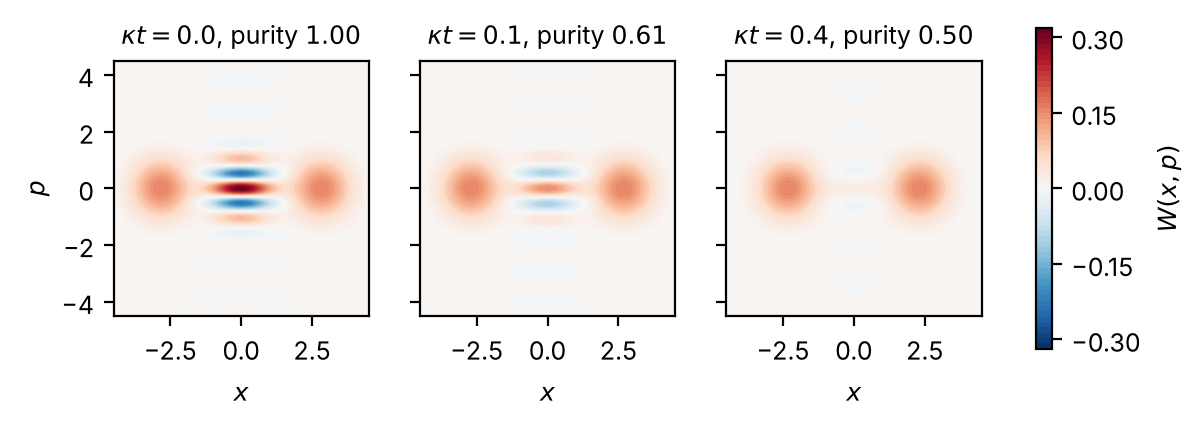
\includegraphics[keepaspectratio,alt={Wigner function of a Schrödinger-cat state under photon loss at three instants: the negative interference fringes disappear while the two coherent components survive. }]{figura_qbasic.png}}
\caption{Wigner function of a Schrödinger-cat state under photon loss at
three instants: the negative interference fringes disappear while the
two coherent components survive. \label{fig:cat}}
\end{figure}

\section{Research impact statement}\label{research-impact-statement}

\textbf{TODO: realized impact.} \emph{List here the research projects,
publications, theses and courses that used Q-BASIC, for example:
``Q-BASIC was used to compute the dynamics reported in (citation) and in
the master's thesis of \ldots{}''; ``the course was taught at \ldots{}
in \ldots{} to \ldots{} students''.}

Q-BASIC has been developed on GitHub since January 2024, and version
0.0.3 has been available on the Python Package Index since December
2024. Version 0.1.0 adds the following evidence of near-term
significance, all verifiable in the repository:

\begin{itemize}
\tightlist
\item
  \textbf{Reproducible materials.} The 15 course notebooks, which cover
  topics such as collapse and revival in the Jaynes-Cummings model
  \citep{eberly1980} and quantum teleportation \citep{bennett1993}, are
  executed by continuous integration and compiled into a PDF book for
  every release; the figure in this paper is regenerated from the
  library by a script in the repository.
\item
  \textbf{Validation.} More than 800 automated tests (98\% line
  coverage) check physical results rather than implementation details:
  Pauli algebra and canonical commutation relations, Poisson statistics
  of coherent states, Rabi and Jaynes-Cummings dynamics against
  analytical solutions and exact diagonalization, spontaneous emission
  and damped oscillators, gate truth tables, and Wigner functions
  against the displaced-parity definition. They run on Linux, Windows
  and macOS with Python 3.10 to 3.14 and with the oldest supported
  dependencies.
\item
  \textbf{Performance.} For a sparse Jaynes-Cummings evolution of
  dimension 400, version 0.1.0 is 26 times faster than version 0.0.x
  with the same Runge-Kutta call, and 177 times faster with the default
  exact propagator; the benchmark script is included.
\end{itemize}

\section{AI usage disclosure}\label{ai-usage-disclosure}

Version 0.0.x of Q-BASIC (2024--2025), including the original simulator,
its operator conventions and the course notebooks, was written by the
author without generative AI. Version 0.1.0 (November 2026) was
developed with Claude Code, an AI coding assistant by Anthropic
(\textbf{TODO: model and version}), working under the author's direction
in the public repository, where the corresponding commits are marked as
co-authored. The assistant was used to reorganize the project as a
package; to rewrite the core class, fix bugs and add the exact
propagator, the Lindblad solver, quantum gates and visualization
functions; to write most of the unit tests, the continuous-integration
workflows and the documentation website; to update the course notebooks
to the new API; to write the script that compiles the notebooks into a
book; and to draft this paper. The author defined the scope and the
structure of the course, approved the design decisions described above
from a written plan, and reviewed, edited and validated all AI-assisted
outputs. Correctness was checked by the physics-based test suite, by
comparison with analytical results, exact diagonalization and QuTiP, and
by executing every notebook of the course.

\section{Acknowledgements}\label{acknowledgements}

\textbf{TODO:} \emph{acknowledge colleagues, students and institutions,
and list any financial support (agency and grant number) with a
statement on whether the sponsor had any involvement in the work, or
state that no specific funding was received.}

\renewcommand\refname{References}
\bibliography{paper.bib}

\end{document}
